\chapterimage{chapter_head_1.pdf} 
\chapter{Fundamentos para programar la NDS}

En este capítulo, se estudiarán los elementos básicos para poder realizar aplicaciones en l consola NDS. En concreto, se estudiarán cuestiones relacionadas con la visualización de texto, la entrada de usuario (botones y pantalla táctil) y el temporizador. 

Para obtener información sobre las funciones existentes, se recomienda ir a la página web: \url{http://libnds.devkitpro.org/}

La lista de ejercicios a realizar y el tiempo estimado (en minutos) para su realización se muestran en la Tabla \ref{c3_tab:ejercios}.

\begin{table}[t]
\centering
\caption{Ejercicios del capítulo y tiempo estimado para su realización.}
\begin{tabular}{|c|c|c|c|}
\hline 
Ejercicio & Tiempo & Ejercicio & Tiempo  \\ 
\hline 
 3.1 & 30'  & 3.11 & 20' \\ 
 3.2 & 10'  & 3.12 & 20' \\ 
 3.3 & 5'   & 3.13 & 10' \\ 
 3.4 & 5'   & 3.14 & 30' \\ 
 3.5 & 10'  & 3.15 & 10' \\ 
 3.6 & 10'  & 3.16 & 10' \\ 
 3.7 & 20'  & 3.17 & 10'\\ 
 3.8 & 15'  & & \\ 
 3.9 & 15'  & & \\ 
 3.10 & 10' & & \\
\hline 
\end{tabular} 
\label{c3_tab:ejercios}
\end{table}
% ---------------------------------------------------------
% ---------------------------------------------------------
\section{Introducción a la programación en NDS}
La estructura básica de las aplicaciones realizadas para NDS es la siguiente:

\begin{lstlisting}
#include [...] 
int main(void)
{
	inicializar libNDS; 
	while(1){
		// Bucle principal 
	}
	return 0;
}
\end{lstlisting}

El bucle infinito sirve para simular el comportamiento de un videojuego al entrar en su bucle principal. El formato habitual de estos tipos de bucles es el siguiente:

\begin{verbatim}
Comienza el bucle:
    Comprobar la entrada de usuario
    Actualizar la lógica interna
    Comprobar el criterio de finalización del bucle
    Redibujar
Fin del bucle
\end{verbatim}



\begin{example}
	El siguiente código muestra un mensaje de texto por la pantalla:
\begin{lstlisting}
#include<nds.h>
#include<stdio.h>
int main(void) {
  consoleDemoInit();
  iprintf("Me gusta programar videojuegos");  // Imprimir el mensaje 
  while(1) 
  {} // Bucle que no hace nada.     
}
\end{lstlisting}
\end{example}


\begin{exercise}
	Crea un nuevo proyecto usando el código anterior para comprobar que tienes bien instalado todo lo necesario para compilar y ejecutar juegos en la NDS. El cápitulo 2 está dedicado a explicar todos los pasos que hay que seguir. 
\end{exercise}

 ---------------------------------------------------------
% ---------------------------------------------------------
\section{Salida de texto}
La Nintendo DS tiene dos pantallas gráficas de tipo LCD (\textit{Liquid Crystal Display}). Las dos tienen el mismo tamaño, 256x192 píxeles, y funcionan gracias a dos motores gráficos: principal o \textit{main} y secundario o \textit{sub}. Además, la pantalla inferior emplea tecnología táctil.

% ---------------------------------------------------------
% ---------------------------------------------------------
\subsection{Visualización de texto en la pantalla}
La pantalla tiene 32 columnas y 24 filas para visualizar texto, tal y como se puede observar en la Figura \ref{fig_c3_texto}. La instrucción \textit{iprintf} se emplea para visualizar texto por la pantalla. Para elegir la posición del texto en la pantalla se usa la secuencia de escape:
\begin{verbatim}
\x1b[<fila>;<columna>H
\end{verbatim}
empleando como valor para la fila un entero entre 0 y 23, y el valor de la columna, un entero entre 0 y 31.

\begin{figure}[t]
\centering
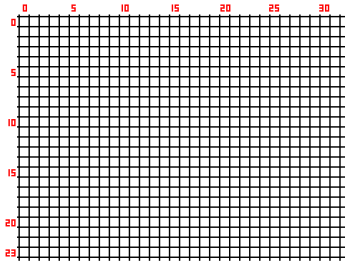
\includegraphics[height=6cm]{Figuras/C3/c3_eclipse12.png}
\caption{Pantalla de la NDS}
\label{fig_c3_texto}
\end{figure}

\begin{example}
El siguiente código muestra un mensaje de texto en la fila 2, columna 5:
\begin{lstlisting}
#include <nds.h>
#include <stdio.h>
int main(void)
{
  consoleDemoInit(); 
  int fila    = 2;
  int columna = 5;
  while(1) {
  	iprintf("\x1b[%d;%dHMensaje de texto", fila, columna);
  	swiWaitForVBlank();  
  }
  return 0;
}
\end{lstlisting}
\end{example}

\begin{exercise}
Realiza un programa que muestre un mensaje de texto aproximadamente en el centro de la pantalla. 
\end{exercise}

\begin{exercise}
Realiza un programa que muestre tres mensajes de texto en varias posiciones diferentes de la pantalla. 
\end{exercise}

% ---------------------------------------------------------
% ---------------------------------------------------------
\subsection{Control de las pantallas a utilizar}
El siguiente programa (\textit{superior.c}) crea una consola para escribir en la pantalla superior:
\begin{lstlisting}
#include <nds.h>
#include <stdio.h>
int main(void)
{
  PrintConsole pantalla;

  videoSetMode(MODE_0_2D);

  consoleInit(
  		&pantalla,        // Consola a inicializar
	    3,                // Capa del fondo donde se imprimirá
	    BgType_Text4bpp,  // Tipo de fondo
	    BgSize_T_256x256, // Tamaño del fondo
	    31,               // Base del mapa
	    0,                // Base del tile gráfico
	    true,             // Sistema grafico a usar (main system)
	    true);            // No cargar gráficos para la fuente

  while(1) {
  iprintf("\x1b[12;10HMensaje de texto");
  swiWaitForVBlank();    // Esperar al refresco de pantalla
  }
  return 0;
}
\end{lstlisting}

En este código cabe destacar lo siguiente:
\begin{itemize}
\item \textit{PrintConsole} es el tipo de datos que define las consolas a utilizar a la hora de imprimir contenidos en pantalla. Se declara la variable \textit{pantalla} de este tipo.
%    
\item La función \textit{VideoSetMode} se encarga de inicializar el sistema gráfico principal (\textit{main}), que es el que se usa en el ejemplo. Si se quiere imprimir en la pantalla inferior, se debería inicializar con \textit{VideoSetModeSub}. Los modos de vídeo soportados (en este caso \textit{MODE\_0\_2D})  dependen del sistema y el fondo que se estén utilizando, y se verán con más detalle en próximos capítulos.
%
\item Para crear una consola con los parámetros deseados se usará la función \textit{consoleInit}. Esta función tiene ocho parámetros de entrada, de los cuales el único que por ahora interesa es el penúltimo que indica el sistema gráfico que se va a usar: con el valor \textit{true}, se utilizará el sistema principal (la pantalla superior), mientras que con el valor \textit{false}, se imprimirá en la pantalla inferior.  \item La función \textit{swiWaitForVBlank} espera al refresco de la pantalla.
\end{itemize}

\begin{exercise}
Crea un nuevo proyecto, usando el programa \textit{superior.c} y comprueba que el resultado obtenido es el esperado.
\end{exercise}

Para usar más de una consola, se deben seguir los pasos del ejemplo anterior, pero además se debe emplear la función \textit{consoleSelect} para indicar qué consola se va a usar. El siguiente programa (\textit{dos\_pantallas.c}) escribe un mensaje en cada una de las pantallas:

\begin{lstlisting}
#include <nds.h>
#include <stdio.h>
int main(void)
{
  PrintConsole pantalla_sup, pantalla_inf;  
  videoSetMode   (MODE_0_2D);
  videoSetModeSub(MODE_0_2D);
  
  consoleInit(&pantalla_sup, 
              3, 
              BgType_Text4bpp,
              BgSize_T_256x256, 
              31, 
              0,
              true, 
              true);
  consoleInit(&pantalla_inf,
              3,
              BgType_Text4bpp,
              BgSize_T_256x256,
              31,
              0,
              false,
              true);

  while(1) {  
   consoleSelect(&pantalla_sup);
   iprintf("\x1b[12;3HEsta es la pantalla superior.");
   consoleSelect(&pantalla_inf);
   iprintf("\x1b[12;3HEsta es la pantalla inferior.");

   swiWaitForVBlank();
  }
  return 0;
}
\end{lstlisting}

\begin{exercise}
Comprueba mediante la creación de un nuevo proyecto, usando el programa \textit{dos\_pantallas.c} que lo indicado ocurre tal y como se comenta. La Figura \ref{p3_c2_dos_pantallas} muestra la salida esperada.
\end{exercise}


\begin{exercise}
	Realiza un programa que muestre tres mensajes en la pantalla superior y otros tres en la pantalla superior.
\end{exercise}

\begin{figure}[t]
\centering
 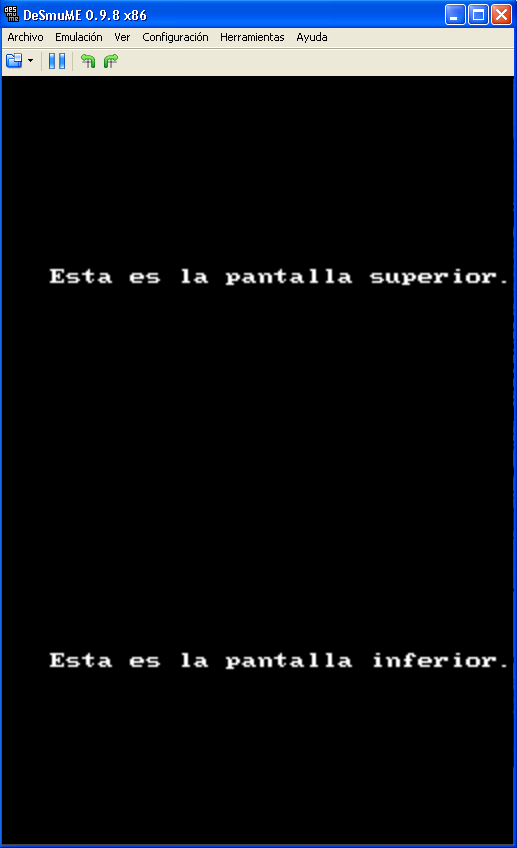
\includegraphics[height=9cm]{Figuras/C3/c3_sol-ejercicios-dospantallas.png}
\caption{Resultado del programa \textit{dos\_pantallas.c}.}
\label{p3_c2_dos_pantallas}
\end{figure}

% ---------------------------------------------------------
% ---------------------------------------------------------
\section{Teclado}
La Nintendo DS tiene la posibilidad de simular el funcionamiento de un teclado empleando funciones de la biblioteca \textit{libnds}. El siguiente programa (\textit{teclado.c}) muestra como funciona el acceso al teclado:

\begin{lstlisting}
#include <nds.h>
#include <stdio.h>
int main(void) {    
  int key;  // Variable que almacena el código ascii de la tecla
    
  consoleDemoInit();  
  keyboardDemoInit();  // Inicializa un teclado
  keyboardShow();      // Visualiza el teclado

  while(1) {       
    key = keyboardUpdate();  // Procesa la tecla pulsada
                             // Retorna el código ascii 
                             // -1 si no se ha pulsado tecla 

    // Visualiza el carácter asociado al ascii de la tecla 
    if (key > 0) iprintf("Tecla pulsada %c \n", key); 

    swiWaitForVBlank(); 
  }
  return 0;
}
\end{lstlisting}

Este programa visualiza la tecla pulsada, para ello se ha introducido el formato \textit{\%c} en la instrucción \textit{iprintf} para visualizar un carácter. La salida del programa \textit{teclado.c} en el emulador se muestra en la Figura \ref{fig_c3_teclado1}.

\begin{figure}[t]
\centering
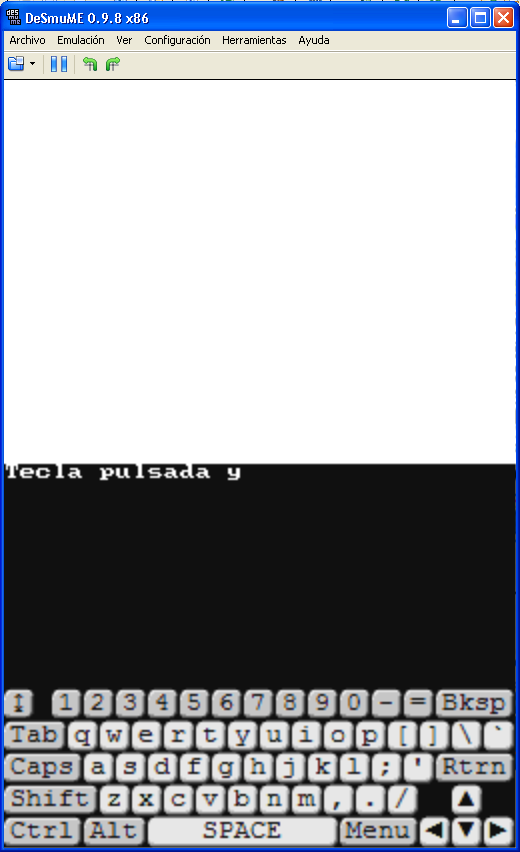
\includegraphics[height=8cm]{Figuras/C3/c3_teclado1.png}
\caption{Salida del programa \textit{teclado.c} en el emulador.}
\label{fig_c3_teclado1}
\end{figure}

En la página web \url{http://libnds.devkitpro.org/keyboard_8h.html} se encuentra más información sobre el funcionamiento del teclado de la NDS.


\begin{exercise}
A partir del código del programa \textit{teclado.c}, crea un programa que muestre tu nombre cuando se pulse una tecla cualquiera y que deje de mostrarlo cuando se deje de pulsar la tecla.
\end{exercise}

\begin{exercise}
A partir del código del programa \textit{teclado.c}, crea un programa que de inicio muestre tu nombre, pero cuando se pulse una tecla cualquiera deje de mostrarlo. Si de nuevo se pulsa una tecla se volverá a mostrar, y así sucesivamente.
\end{exercise}

\begin{exercise}
A partir del código del programa \textit{teclado.c}, crea un programa que muestre tu nombre cuando se pulse la tecla \textit{s}. El nombre continuará visible hasta que se pulse la tecla \textit{n}. Si se vuelve a pulsar la tecla \textit{s}, el nombre volverá a ser visible y así sucesivamente.
\end{exercise}

% ---------------------------------------------------------
% ---------------------------------------------------------
\section{Botones de la consola}
La consola NDS presenta los siguientes botones como entrada de usuario (ver Figura \ref{fig_c3_botones}):
\begin{itemize}
\item Una cruceta direccional a la izquierda de la pantalla inferior (cruceta de 4 direcciones).
%
\item Cuatro botones (\textit{A}, \textit{B}, \textit{X}, \textit{Y}) a la derecha de la pantalla inferior.
%
\item Dos botones laterales (\textit{L} y \textit{R}) situados detrás.
%
\item Botón de \textit{Select} y botón de \textit{Start}, a la derecha de la pantalla inferior.
%
\item La pantalla táctil inferior.
\end{itemize}

\begin{figure}[t]
\centering
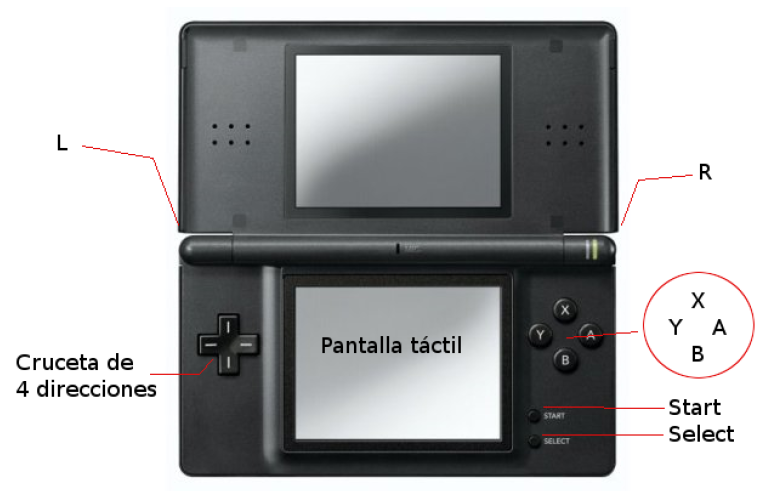
\includegraphics[height=7cm]{Figuras/C3/c3_botones.png}
\caption{Botones de la NDS.}
\label{fig_c3_botones}
\end{figure}

Además, el cierre de la consola tiene también un sensor para saber si está abierta o cerrada, que a efectos de programación, funciona como otro botón más.

La Figura \ref{fig_c3_botones_teclass} muestra la relación que existe entre los botones de la NDS y el teclado en el emulador.

\begin{figure}[t]
\centering
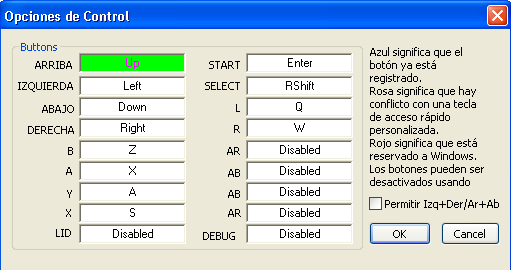
\includegraphics[height=5.5cm]{Figuras/C3/c3_botones_teclas.png}
\caption{Relación que existe entre los botones de la NDS y el teclado.}
\label{fig_c3_botones_teclass}
\end{figure}

Los pasos a seguir para determinar las operaciones realizadas con los botones son las siguientes:
\begin{enumerate}
\item Primero, en cada paso por el bucle principal, se determinará si se ha pulsado algunos de los botones mediante la función \textit{scanKeys}. 
%
\item Después se puede  obtener información sobre los botones con las siguientes funciones:
\begin{itemize}
	\item \textit{keysCurrent}: obtiene el estado actual de los botones.
	\item \textit{keysDown}: obtiene los botones pulsados en ese instante.
	\item \textit{keysHeld}: obtiene los botones mantenidos.
	\item \textit{keysUp}: obtiene los botones liberados.
\end{itemize}
\end{enumerate}

El resultado de estas funciones se compara mediante una \textit{multiplicación bit a bit} con el valor del botón del que se quiere saber su estado. Como valores del botón cuyo estado se desea saber se puede emplear: 
\begin{itemize}
\item Los cuatro botones de la derecha: KEY\_A, KEY\_B, KEY\_X, KEY\_Y.
\item Los botones laterales \textit{L} y \textit{R}: KEY\_L, KEY\_R.
\item Botones \textit{Select} y \textit{Start}: KEY\_SELECT, KEY\_START.
\item La cruceta de 4 direcciones: KEY\_UP, KEY\_DOWN, KEY\_LEFT, KEY\_RIGHT.
\item La pantalla táctil (solo como botón): KEY\_TOUCH.
\item La bisagra del cierre de la consola: KEY\_LID.
\end{itemize}

La siguiente página web contiene informaicón sobre el uso de la botonera \url{http://libnds.devkitpro.org/arm9_2input_8h.html}

El siguiente ejemplo (\textit{botones.c}) comprueba el estado instantáneo de cada botón, mostrando en pantalla si se ha pulsado: 
\begin{lstlisting}
#include <nds.h>
#include <stdio.h>
int main()
{
  u32 keys;
  consoleDemoInit();

  while(1){
    scanKeys();
    keys = keysCurrent(); // Se lee el estado actual de todos los botones

    // Se comprueba si se ha pulsado arriba en la cruceta
    if (keys & KEY_UP) iprintf("\x1b[10;5H Pulsado UP");
    else               iprintf("\x1b[10;5H           ");

   // Se comprueba si se ha pulsado en el boton A
   if (keys & KEY_A)   iprintf("\x1b[12;5H Pulsado A");
   else                iprintf("\x1b[12;5H          ");

   // Se comprueba si se ha pulsado el botón Start
   if (keys & KEY_START) iprintf("\x1b[15;5H Pulsado START");
   else                  iprintf("\x1b[15;5H              ");

   // Se comprueba si se ha pulsado la pantalla táctil
   if (keys & KEY_TOUCH) iprintf("\x1b[13;5H Pantalla tactil");
   else                  iprintf("\x1b[13;5H                ");

   swiWaitForVBlank();
  }
  return 0;
}
\end{lstlisting}

Se puede observar que se llama a la función \textit{scanKeys}, posteriormente se llama a la función \textit{keysCurrent} para conocer el estado actual de los botones. Dicha información se guarda en la variable \textit{keys}, declarada de tipo \textit{u32} (entero sin signo de 32 bits). Con el valor de esta variable se realiza la multiplicación bit a bit con el valor de un botón específico mediante:
\begin{lstlisting}
if (keys & KEY_UP)
\end{lstlisting}

Si el botón está pulsado, se muestra en pantalla un mensaje indicando el  botón en concreto, incluyendo la pantalla táctil. Si se quieren realizar
acciones en momentos precisos (justo cuando se pulsa un botón, o cuando se libera), se podrán utilizar el resto de funciones.

\begin{exercise}
Comprueba mediante la creación de un nuevo proyecto, usando el código \textit{botones.c}, que lo indicado ocurre tal y como se comenta.
\end{exercise}

\begin{exercise}
Realiza un programa que permita desplazar un mensaje de texto por la pantalla inferior empleando los botones de dirección (derecha, izquierda, arriba y abajo). Se debe controlar que el mensaje completo siempre se encuentre dentro de la pantalla, y que se desplace solo una posición en cada pulsación del correspondiente botón.
\end{exercise}

\begin{exercise}
Modifica el programa anterior para que al pulsar el botón \textit{X} se cambie el mensaje a mostrar por otro mensaje. Al pulsar el botón \textit{B} se deberá volver a mostrar el mensaje original.
\end{exercise}

% ---------------------------------------------------------
% ---------------------------------------------------------
\section{Pantalla táctil}
\label{sec_pantalla_tactil}
Como ya se ha comentado, la pantalla inferior emplea tecnología táctil. En la Nintendo DS se usa el  sistema de coordenadas cartesiano mostrado en la Figura \ref{fig_c3_cartesiano}. En el emulador se emplea el ratón como puntero de la pantalla táctil.

La siguiente página web contiene informaicón sobre el uso de la pantalla táctil  \url{http://libnds.devkitpro.org/arm9_2input_8h.html}

El siguiente programa (\textit{tactil.c}) cuenta el número de veces que se pulsa en la pantalla táctil.

\begin{figure}[t]
\centering
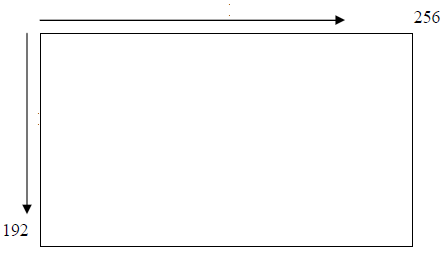
\includegraphics[height=7cm]{Figuras/C3/c3_coordenadas.png}
\caption{Sistema de coordenadas cartesiano usado para detectar donde ha pulsado el usuario en la pantalla táctil.}
\label{fig_c3_cartesiano}
\end{figure}

\begin{lstlisting}
#include <nds.h>
#include <stdio.h>

int main(void) {
  touchPosition posicionXY;
  int           contador;

  consoleDemoInit();
  contador = 0;

  while(1)
  {
    scanKeys();
    touchRead(&posicionXY); // Se lee la posición actual.
    iprintf("\x1b[1;0HPosicion x=%04i y=%04i ",
            posicionXY.px, 
            posicionXY.py);
    iprintf("\x1b[2;0HContador=%04i", 
            contador);

    if (keysDown() & KEY_TOUCH) contador++;

    swiWaitForVBlank();
  }
  return 0;
}
\end{lstlisting}

De este código se puede destacar lo siguiente:
\begin{itemize}
\item Se crea una variable del tipo \textit{touchPosition} (en este caso \textit{posicionXY}) para reconocer la posición del puntero en la pantalla táctil. Mediante \textit{posicionXY.px} se obtiene la posición respecto al eje \textit{x}, mientras que con \textit{posicionXY.py} se obtiene la posición respecto al eje \textit{y}.
%
\item La función \textit{touchRead} lee el valor de la posición del puntero en la pantalla táctil.
%
\item El formato \textit{\%04i} en la instrucción \textit{iprintf}  visualiza un número entero de 4 cifras (en decimal)  poniendo ceros en la izquierda. 
\end{itemize}

\begin{exercise}
	Comprueba mediante la creación de un nuevo proyecto, usando el código \textit{tactil.c}, que lo indicado ocurre tal y como se comenta.
\end{exercise}

\begin{exercise}
Realiza un programa que divida la pantalla inferior en 4 zonas. En cada una de ellas deberá aparecer un contador que contará el número de veces que se pulsa en cada zona. La Figura \ref{fig_p3_c3_4zonas} muestra un ejemplo de la salida del programa requerido.
\end{exercise}

\begin{figure}[t]
\centering
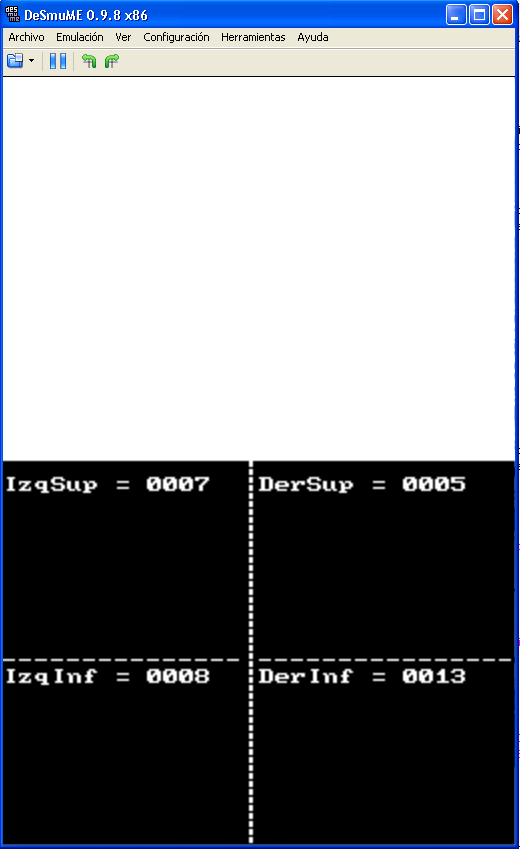
\includegraphics[height=7.5cm]{Figuras/C3/c3_tactil1.png}
\caption{Salida ejemplo del programa requerido en la sección \ref{sec_pantalla_tactil}}
\label{fig_p3_c3_4zonas}
\end{figure}

% ---------------------------------------------------------
% ---------------------------------------------------------
\section{Temporizador}
La Nintendo DS cuenta con temporizadores (\textit{timers}) de tiempo real, que pueden ser empleados por una aplicación o juego para definir diferentes respuestas dependiendo de la hora del día. Las características que tienen son las siguientes:

\begin{itemize}
	\item Hay 8 temporizadores de 16 bits, 4 en el ARM9 y 4 en el ARM7.
	\item Funcionan como contadores de eventos.
	\item La frecuencia base con la que trabajan es de 33MHz, sobre la que se puede aplicar los siguientes divisores de frecuencia: 1, 64, 256 y 1024.
	\item Soportan la configuración en cascada, es decir, que cuando un temporizador se desborda el si\-guien\-te temporizador incrementa su cuenta.
	\item Pueden generar interrupciones. 
\end{itemize}

La página web \url{http://libnds.devkitpro.org/timers_8h.html} muestra información sobre los temporizadores.

El siguiente programa (\textit{tiempo.c}) muestra el tiempo que va transcurriendo en segundos:
\begin{lstlisting}
#include <nds.h>
#include <stdio.h>
#include <time.h>
//se define la velocidad del reloj con ClockDivider_1024
#define TIMER_SPEED (BUS_CLOCK/1024)
int main()
{
  consoleDemoInit();
  uint ticks = 0;
  timerStart(0, ClockDivider_1024, 0, NULL); // Iniciar el reloj
  while (1)
  {
   ticks += timerElapsed(0);  
   iprintf("\x1b[1;0Hticks:  %u",ticks);
   iprintf("\x1b[2;0Hseg.: %u:%u",
           ticks/TIMER_SPEED,
           ((ticks%TIMER_SPEED)*1000)/TIMER_SPEED);
   swiWaitForVBlank();
  }
  return 0;
}
\end{lstlisting}

Se declara la variable \textit{ticks} como \textit{uint} (entero sin signo). En la llamada \textit{timerStart} cabe destacar lo si\-guien\-te:
\begin{itemize}
\item El primer parámetro hace referencia al \textit{temporizador 0}.
%
\item El parámetro \textit{ClockDivider\_1024} hace referencia a aplicar una división de frecuencia de 1024.
\end{itemize}

La función \textit{timerElapsed} proporciona el número de ticks que se han producido desde la última llamada a esa misma función, para el temporizador especificado (en este caso el 0).  El formato \textit{\%u} en la instrucción \textit{iprintf}  visualiza un número entero sin signo.

\begin{exercise}
	Comprueba mediante la creación de un nuevo proyecto, usando el código \textit{tiempo.c}, que lo indicado ocurre tal y como se comenta.
\end{exercise}

\begin{exercise}
Modifica el programa \textit{tiempo.c} para que finalice la cuenta si han transcurrido 15 segundos o si se ha pulsado el boton \textit{Y}.
\end{exercise}

En ocasiones se desea que ocurra un evento cada cierto tiempo. Por ejemplo, el siguiente código (eventos.c) mueve la letra \textit{X} hacia la derecha cada 2 segundos:

\begin{lstlisting}
#include <nds.h>
#include <stdio.h>
#include <time.h>

#define TIMER_SPEED (BUS_CLOCK/1024)

int main()
{
  consoleDemoInit();
  uint ticks = 0;
  int posicion = 0;
  int segundos;
  int proximo_cambio = 2;

  timerStart(0, ClockDivider_1024, 0, NULL);

  while (1)
  {
    ticks += timerElapsed(0);
    segundos = (int) (ticks/TIMER_SPEED);

    if (segundos >= proximo_cambio)
    {
      posicion = posicion + 1;
      proximo_cambio = proximo_cambio + 2;
    }
    iprintf("\x1b[1;%dH ",posicion-1);
    iprintf("\x1b[1;%dHX",posicion);
    swiWaitForVBlank();
  }
  return 0;
}
\end{lstlisting}

\begin{exercise}
	Modifica el programa \textit{evento.c} para que la letra se mueva cada 3 segundos.
\end{exercise}

Es importante destacar que para programar este tipo de funcionalidad, es más conveniente el uso de interrupciones, tal como se verá posteriormente.

